\section{实验}
\label{sec:exp}

\subsection{实验设置}
\label{sec:setup}

\textbf{数据与协议。}全部实验采用第~\ref{sec:bench} 节的 TrajGap-Bench Mixed 协议：Mixed-train 用于拟合，Mixed-val 用于按最终预测头的 $\mathrm{minFDE}_{20}$ 选择检查点，Mixed-test 仅评估一次；五个场景，$T=8$，$H=12$，$K=20$。依照数据发布的逐场景划分，每个场景训练一个模型。所有方法均在自然的 Mixed 分布上训练，不按缺失帧数重新加权。

\textbf{实现细节。}GAST 的嵌入宽度为 128，注意力头数为 8，时间栈包含四层选择性状态空间块，解码器含两层交叉注意力，$K=20$，dropout 与 drop-path 均为 0.2。训练使用 AdamW，学习率 $10^{-3}$，权重衰减 $10^{-4}$，预热 5 个轮次，梯度裁剪范数 5，批大小 64，bf16 混合精度，最多 100 个轮次；实际选中的检查点位于第 33 至 58 轮之间，故训练预算不构成约束。每个场景使用单张 NVIDIA RTX 5880 Ada GPU 训练。模型参数量为 1.19M。所有方法的随机种子固定为 2024。

\textbf{对比方法。}本文与六种外部方法对比，覆盖两类。
\begin{itemize}
\item \emph{完整历史预测器。}\textbf{SocialLSTM} \cite{alahi2016social} 采用缺失感知变体（零占位、缺失帧跳过 LSTM 状态更新、$K=20$ 的高斯混合头）。\textbf{AgentFormer} \cite{yuan2021agentformer} 接收逐帧有效性通道，并以最后观测帧作为解码锚点。\textbf{MoFlow} \cite{fu2025moflow} 使用官方实现，配以掩码感知特征，缺失步以逐通道均值占位。\textbf{Re} \cite{mao2025resonance} 以零填充历史原样运行。
\item \emph{插补感知与图结构预测器。}\textbf{MS-TIP} \cite{chib2024mstip} 将基于 SAITS 的插补分支与预测器耦合、端到端训练，代表直接输入约束下的“插补—预测”路线。\textbf{Social-STGCNN} \cite{mohamed2020social} 作为图结构参照，缺失行人被表示为既不发送也不接收消息的幽灵节点。
\end{itemize}
不具备模式概率头的方法（AgentFormer、Re、MS-TIP、Social-STGCNN）不参与 top-1 诊断，但参与仅需 $K$ 条候选的主指标。所有方法读取完全相同的测试张量。

\subsection{主要结果}
\label{sec:main}

表~\ref{tab:main} 给出主对比结果。GAST 在两项指标上均取得最优宏平均（0.3168/0.4831~m）与最优微平均（0.2894/0.4716~m）。相对最强外部基线（MoFlow），宏平均上 $\mathrm{minADE}_{20}$ 降低 9.4\%、$\mathrm{minFDE}_{20}$ 降低 7.6\%，微平均上降低 7.5\%/5.3\%。GAST 在 $\mathrm{minADE}_{20}$ 上对 MoFlow 五个场景全胜，在 $\mathrm{minFDE}_{20}$ 上四胜一负，唯一例外是 ZARA1-M，MoFlow 在该场景优 1.8\%。

逐场景结果比聚合值更能说明问题。GAST 在 ETH-M、UNIV-M、ZARA1-M 与 ZARA2-M 上取得最优 $\mathrm{minADE}_{20}$，在 ETH-M、UNIV-M 与 ZARA2-M 上取得最优 $\mathrm{minFDE}_{20}$。在 HOTEL-M 上 AgentFormer 明显更优（0.2083/0.3316 对 0.2541/0.3769），在 ZARA1-M 的 $\mathrm{minFDE}_{20}$ 上 MoFlow 略优（0.4057 对 0.4128）。可见 GAST 的优势并不覆盖所有场景，其宏平均领先来自 ETH-M 与 UNIV-M 上较大幅度的收益；第~\ref{sec:disc} 节讨论何种场景特征与方法收益相关。

两种最弱的基线差距明显。MS-TIP 作为插补感知联合训练的代表位列倒数第二，以幽灵节点表示缺失行人的 Social-STGCNN 位列末位。二者与其他方法遵循同一评测契约，因此差距并非协议造成；它反映的是 8 帧历史、最多缺失七帧且缺口频繁延伸至预测起点这一设定的难度。经典社会池化模型同样明显落后（0.4576/0.6079），考虑到历史很短且其缺失感知变体缺乏显式多模态建模，这一结果在预期之内。

\begin{table*}[t]
\centering
\scriptsize
\setlength{\tabcolsep}{2.4pt}
\caption{TrajGap-Bench Mixed-test 主结果（$K=20$，随机种子 2024）。单元格为 $\mathrm{minADE}_{20}$/$\mathrm{minFDE}_{20}$，单位米，越低越好。Macro 为五场景宏平均，Micro 为按测试样本数加权的微平均。逐场景、逐指标最优加粗。标 $\dagger$ 的方法输出无权重样本，不参与 top-1 诊断。}
\label{tab:main}
\begin{tabular}{@{}lccccccc@{}}
\toprule
Method & ETH-M & HOTEL-M & UNIV-M & ZARA1-M & ZARA2-M & Macro & Micro \\
\midrule
\textbf{GAST (ours)} & \textbf{0.5852}/\textbf{0.8212} & 0.2541/0.3769 & \textbf{0.3200}/\textbf{0.5244} & \textbf{0.2510}/0.4128 & \textbf{0.1738}/\textbf{0.2801} & \textbf{0.3168}/\textbf{0.4831} & \textbf{0.2894}/\textbf{0.4716} \\
MoFlow & 0.6819/0.9389 & 0.2777/0.4247 & 0.3478/0.5572 & 0.2566/\textbf{0.4057} & 0.1839/0.2867 & 0.3496/0.5227 & 0.3129/0.4981 \\
AgentFormer & 0.7098/1.0436 & \textbf{0.2083}/\textbf{0.3316} & 0.4132/0.6796 & 0.3551/0.5795 & 0.2690/0.4375 & 0.3911/0.6144 & 0.3795/0.6220 \\
SocialLSTM & 0.8430/1.0456 & 0.2924/0.3871 & 0.4543/0.6512 & 0.4126/0.5650 & 0.2858/0.3907 & 0.4576/0.6079 & 0.4193/0.5941 \\
Re$^{\dagger}$ & 0.9945/1.4262 & 0.7799/1.2808 & 0.5388/0.8408 & 0.4960/0.7470 & 0.3819/0.5928 & 0.6382/0.9775 & 0.5187/0.8085 \\
MS-TIP$^{\dagger}$ & 1.6345/2.0985 & 1.3102/1.5472 & 1.3240/1.1566 & 0.8842/1.1720 & 0.7663/0.9902 & 1.1838/1.3929 & 1.1991/1.1461 \\
Social-STGCNN$^{\dagger}$ & 2.1393/3.5048 & 1.3022/2.1624 & 0.9496/1.5336 & 1.4801/2.7038 & 0.8646/1.5258 & 1.3471/2.2861 & 0.9878/1.6409 \\
\bottomrule
\end{tabular}
\end{table*}

\subsection{缺失程度增加下的行为}
\label{sec:severity}

表~\ref{tab:severity} 与图~\ref{fig:degrad} 按历史缺失帧数对测试集分层。基准的官方扫描使缺失 $0$ 至 $7$ 帧的每个桶在测试集上等权（每桶 33{,}654 个样本；缺失四帧的桶为 67{,}308，因为 ETH-M 在该桶贡献了两份），因此各桶可直接比较。

各曲线在聚合值之外给出更清晰的分离。GAST 在缺失零至六帧区间退化最平缓：$\mathrm{minFDE}_{20}$ 由 0.3592 升至 0.4281~m（$+19\%$），而 MoFlow 由 0.3793 升至 0.5534~m（$+46\%$）。相对 MoFlow 的优势并非常数，而是随严重程度扩大：缺失零帧时 $-5.4\%$，三帧时 $-11.2\%$，五帧时 $-14.8\%$，六帧时 $-22.6\%$；$\mathrm{minADE}_{20}$ 上对应的变化为 $-6.7\%$ 至 $-25.9\%$。这一“剂量—效应”形态与证据条件化的设计意图一致，即收益应随可用证据减少而增大。

缺失七帧时仅剩一个观测。此时排序发生反转：MoFlow 的 $\mathrm{minFDE}_{20}$ 为 1.2224~m，优于 GAST 的 1.2731~m（$+4.1\%$）；$\mathrm{minADE}_{20}$ 上 MoFlow 亦更优（0.8734 对 0.9126）。只有一帧时不存在可利用的速度、朝向与缺口结构，预测由学习到的先验决定，为证据路由而正则化的模型已无证据可路由。本文将其视为该区间的边界而非模型失效，但这确实意味着不应宣称 GAST 改善了单帧情形。

\begin{table*}[t]
\centering
\footnotesize
\setlength{\tabcolsep}{4.6pt}
\caption{按历史缺失帧数分层的结果（五场景宏平均，单位米）。除缺失四帧为 67{,}308 个样本外，其余各桶均为 33{,}654 个样本。各桶最优值加粗。}
\label{tab:severity}
\begin{tabular}{@{}lcccccccc@{}}
\toprule
 & 0 & 1 & 2 & 3 & 4 & 5 & 6 & 7 \\
\midrule
\multicolumn{9}{@{}l}{\emph{$\mathrm{minADE}_{20}$}}\\
GAST & \textbf{0.2154} & \textbf{0.2192} & \textbf{0.2286} & \textbf{0.2336} & \textbf{0.2440} & \textbf{0.2629} & \textbf{0.2911} & 0.9126 \\
MoFlow & 0.2309 & 0.2390 & 0.2481 & 0.2706 & 0.2847 & 0.3221 & 0.3926 & \textbf{0.8734} \\
\midrule
\multicolumn{9}{@{}l}{\emph{$\mathrm{minFDE}_{20}$}}\\
GAST & \textbf{0.3590} & \textbf{0.3632} & \textbf{0.3756} & \textbf{0.3777} & \textbf{0.3854} & \textbf{0.4002} & \textbf{0.4281} & 1.2731 \\
MoFlow & 0.3793 & 0.3889 & 0.3968 & 0.4254 & 0.4341 & 0.4695 & 0.5534 & \textbf{1.2224} \\
\bottomrule
\end{tabular}
\end{table*}

\begin{figure*}[t]
\centering
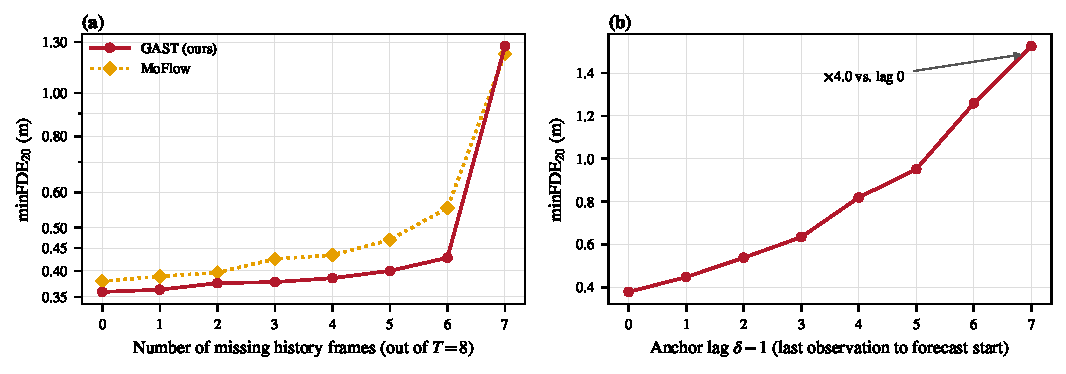
\includegraphics[width=\textwidth]{figures/degradation_en.pdf}
\caption{退化与证据损失（五场景宏平均）。(a) $\mathrm{minFDE}_{20}$ 随历史缺失帧数的变化，纵轴为对数刻度；缺失七帧处反映仅剩一次观测的区间变化。(b) $\mathrm{minFDE}_{20}$ 随锚点间隔（末次观测到预测起点的步数）的变化，间隔 7 处的误差约为间隔 0 的 4.0 倍。}
\label{fig:degrad}
\end{figure*}

\subsection{末端缺失与锚点间隔}
\label{sec:lag}

表~\ref{tab:lag} 沿两个被缺失计数混淆的轴描述 GAST 的误差结构。末端缺失把缺口延伸至预测起点的样本与缺口提前结束的样本分开，锚点间隔则计数末次观测到起点的步数。由于公开基线未提供相同粒度的分层预测，本节仅报告 GAST 自身的分层结果，用于刻画误差随证据年龄的增长方式。

误差随锚点间隔单调上升：$\mathrm{minFDE}_{20}$ 从间隔 0 的 0.3787~m 增至间隔 7 的 1.5260~m，约为前者的 4.0 倍；$\mathrm{minADE}_{20}$ 由 0.2272~m 增至 1.1847~m。增长并非线性：间隔 0 至 2 每增加一步约抬升 18\%–42\%，间隔 3 之后每步抬升幅度更大，至间隔 7 达到 303\%。这表明当末次观测远离预测起点时，误差主要由锚点状态的陈旧程度决定，而非由场景差异决定。

末端缺失组的 $\mathrm{minFDE}_{20}$ 为 0.6112~m，比非末端组的 0.3787~m 高 61.4\%；$\mathrm{minADE}_{20}$ 相应高 87.9\%。这正是锚点状态与进度参数化骨架所针对的条件：缺口延伸至起点时，首个预测点必须从陈旧的锚点出发，且其后的未观测区间完全不可见。间隔 7 处的极端值提示可靠度衰减应在某一年龄之后饱和，而不是持续偏好极旧的状态；本文将这一点作为当前形式的局限而非调优结果。

\begin{table}[t]
\centering
\footnotesize
\setlength{\tabcolsep}{3.4pt}
\caption{GAST 按锚点间隔与末端缺失分层的结果（五场景宏平均）。单元格为 $\mathrm{minADE}_{20}$/$\mathrm{minFDE}_{20}$，单位米；$\Delta$ 为相对锚点间隔 0 的 $\mathrm{minFDE}_{20}$ 变化，非末端组与间隔 0 为同一批样本。}
\label{tab:lag}
\begin{tabular}{@{}l c c r@{}}
\toprule
Group & $n$ & GAST & $\Delta$FDE \\
\midrule
lag 0 & 167{,}469 & 0.2272/0.3787 & --- \\
lag 1 & 60{,}284 & 0.2887/0.4480 & $+18.3\%$ \\
lag 2 & 30{,}263 & 0.3581/0.5384 & $+42.2\%$ \\
lag 3 & 17{,}368 & 0.4477/0.6345 & $+67.6\%$ \\
lag 4 & 10{,}763 & 0.6051/0.8195 & $+116.4\%$ \\
lag 5 & 7{,}379 & 0.7564/0.9515 & $+151.3\%$ \\
lag 6 & 5{,}356 & 0.9577/1.2590 & $+232.5\%$ \\
lag 7 & 4{,}004 & 1.1847/1.5260 & $+303.0\%$ \\
\midrule
terminal & 135{,}417 & 0.4268/0.6112 & $+61.4\%$ \\
\bottomrule
\end{tabular}
\end{table}

\subsection{覆盖度与排序}
\label{sec:coverage}

表~\ref{tab:top1} 报告 top-1 诊断。GAST 的 $\mathrm{ADE@1}$/$\mathrm{FDE@1}$ 为 0.9806/1.7887~m，与 MoFlow 的 0.9814/1.7296~m 基本相当：$\mathrm{ADE@1}$ 略优 0.1\%，$\mathrm{FDE@1}$ 略差 3.4\%；相对 SocialLSTM 则分别优 26.1\% 与 18.2\%。将这一结果与主指标对照可知，GAST 相对 MoFlow 在 best-of-20 上取得的 9.4\%/7.6\% 提升并未同步体现在概率最高的单一模式上。

这一分离对使用方式有直接影响。best-of-20 衡量的是候选集合对真实未来的覆盖能力，而部署在规划器之后的预测器通常只消费概率最高的模式。因此 GAST 的收益更适用于对候选集合做保守规划或集成的场合；若下游仅依赖 top-1，则其相对 MoFlow 的优势将收窄至统计噪声量级。排序质量的改进需要单独设计模式评分目标，本文未对此作进一步处理，并将其列为开放问题。

\begin{table}[t]
\centering
\footnotesize
\setlength{\tabcolsep}{4.2pt}
\caption{top-1 诊断（宏平均，单位米）。$\mathrm{ADE@1}$/$\mathrm{FDE@1}$ 取概率最高的模式。无模式概率的方法未列入。}
\label{tab:top1}
\begin{tabular}{@{}lcc@{}}
\toprule
Method & $\mathrm{ADE@1}$ & $\mathrm{FDE@1}$ \\
\midrule
GAST & \textbf{0.9806} & 1.7887 \\
MoFlow & 0.9814 & \textbf{1.7296} \\
SocialLSTM & 1.3278 & 2.1865 \\
\bottomrule
\end{tabular}
\end{table}

\subsection{可复现性}
\label{sec:repro}

评测协议、Mixed 适配器、训练入口、评估器与模型配置以单一代码仓库发布。每次运行写出 manifest，记录 git 版本、解析后的配置、所消费的数据文件、检查点规则与环境信息（Python、PyTorch 与 CUDA 版本）。评估输出一个 JSON 文件，包含五个分层维度的逐样本诊断；本文全部表格由脚本从这些文件生成，而非手工转抄。Laplace 似然存在两种数值等价的实现，其中一种为向量化版本；等价性门禁校验二者梯度在机器精度内一致，每次运行实际使用的实现记录在其 manifest 中。
